\documentclass[conference,10pt]{IEEEtran}
\usepackage[cmex10]{amsmath}
\usepackage{amsthm,amsfonts,mathrsfs}
\usepackage{graphicx}
\usepackage{dsfont,enumitem,stackrel}
\usepackage{color}
\usepackage{mathtools,amssymb,bm,mathabx}
\usepackage{amstext}
\usepackage{array}
\usepackage{algorithmicx}
\usepackage[ruled]{algorithm}
\usepackage{algpseudocode}
\usepackage{algpascal}
\usepackage{algc}
\usepackage{subfigure}
\usepackage{cases}
\usepackage{pgfplots}
\pgfplotsset{compat=newest}
\usetikzlibrary{spy}
\usepackage{accents}
\usepackage{float}
\usepackage{cite}
\usepackage{hyperref}
\usepackage[nolist,withpage]{acronym}
\usepackage{etoolbox}
\makeatletter
\newif\if@in@acrolist
\AtBeginEnvironment{acronym}{\@in@acrolisttrue}
\newrobustcmd{\LU}[2]{\if@in@acrolist#1\else#2\fi}

\newcommand{\ACF}[1]{{\@in@acrolisttrue\acf{#1}}}
\makeatother


\theoremstyle{remark}
\renewcommand{\qedsymbol}{$\blacksquare$}
\newcommand{\myhyperref}[2]{#2 \ref{#1}}
\newcommand{\vect}[2]{\left[ #1_1, #1_2, #1_3, ..., #1_#2 \right]^{\mathsf{T}}}
\newcommand*{\Scale}[2][4]{\scalebox{#1}{$#2$}}%
\newcommand*{\Resize}[2]{\resizebox{#1}{!}{$#2$}}%
\newcommand{\alg}{\texttt{algorithmicx}}
\newcommand{\old}{\texttt{algorithmic}}
\newcommand{\euk}{Euclid}
\newcommand\ASTART{\bigskip\noindent\begin{minipage}[b]{0.5\linewidth}}
	\newcommand\ACONTINUE{\end{minipage}\begin{minipage}[b]{0.5\linewidth}}
	\newcommand\AENDSKIP{\end{minipage}\bigskip}
\newcommand\AEND{\end{minipage}}
\newcommand{\RN}[1]{%
	\textup{\uppercase\expandafter{\romannumeral#1}}%
}



\def\C{ \mathbb{C}}
\def\R{\mathbb{R}}
\def\Z{ \mathbb{Z}}
\def\N{ \mathbb{N}}
\def\change{red}
\theoremstyle{plain}
\newtheorem{thm}{\textbf{Theorem}}
\newtheorem{lem}{\textbf{Lemma}}
\newtheorem{prop}{\textbf{Proposition}}
\newtheorem*{corl}{\textbf{Corollary}}
\newtheorem{result}{\textbf{Result}}
\theoremstyle{definition}
\newtheorem{defn}{\textbf{Definition}}
\newtheorem{conj}{\textbf{Conjecture}}
\newtheorem{example}{\textbf{Example}}
\theoremstyle{remark}
\newtheorem{rem}{\bf Remark}
\newtheorem*{sketch}{\bf Proof skech }
\newtheorem*{note}{Note}
\newcommand*{\rom}[1]{\expandafter\@slowromancap\romannumeral #1@}





\definecolor{azure}{rgb}{0.0, 0.5, 1.0}
\definecolor{ashgrey}{rgb}{0.7, 0.75, 0.71}
\definecolor{chestnut}{rgb}{0.8, 0.36, 0.36}
\definecolor{airforceblue}{rgb}{0.36, 0.54, 0.66}
\definecolor{cadmiumorange}{rgb}{0.93, 0.53, 0.18}
\definecolor{bleudefrance}{rgb}{0.19, 0.55, 0.91}
\definecolor{carolinablue}{rgb}{0.6, 0.73, 0.89}
\definecolor{blue(ncs)}{rgb}{0.0, 0.53, 0.74}
\definecolor{dodgerblue}{rgb}{0.12, 0.56, 1.0}
\definecolor{cssgreen}{rgb}{0.0, 0.5, 0.0}
\definecolor{cadmiumgreen}{rgb}{0.0, 0.42, 0.24}
\definecolor{cadmiumorange}{rgb}{0.93, 0.53, 0.18}
\definecolor{amaranth}{rgb}{0.9, 0.17, 0.31}
\definecolor{bluegray}{rgb}{0.4, 0.6, 0.8}
\definecolor{cadmiumgreen}{rgb}{0.0, 0.42, 0.24}











% Example definitions.
% --------------------
\def\x{{\mathbf x}}
\def\L{{\cal L}}

% Title.
% ------
\title{Gridless Blind Deconvolution and Demixing}
% \author{Saeed~Razavikia, Sajad~Daei, Carlo Fischione }%
%
% Single address.
% ---------------
\author{\IEEEauthorblockN{Saeed Razavikia, Sajad Daei, Mikael Skoglund, Gabor Fodor, Carlo Fischione}
 \IEEEauthorblockA{School of Electrical Engineering and Computer Science, KTH Royal Institute of Technology, Stockholm, Sweden\\
Email: \{sraz, sajado, skoglund, gaborf, carlofi\}@kth.se}
}



\begin{document}
\bstctlcite{IEEEexample:BSTcontrol}
\maketitle
\newacronym{DAC}{DAC}{Digital to Analog Converter}
\newacronym{DC}{DC}{Direct Current}
\newacronym{DRIE}{DRIE}{Deep Reactive Ion Etching}
\newacronym{IMSL}{IMSL}{Inverted MicroStrip Line}
\newacronym{ITO}{ITO}{Indium Tin Oxide}
\newacronym{LCD}{LCD}{Liquid Crystal Display}
\newacronym{LOS}{LOS}{Line-Of-Sight}
\newacronym{MEMS}{MEMS}{Micro-Electro-Mechanical Systems}
\newacronym{mm-Wave}{mm-Wave}{millimeter-Wave}
\newacronym{NLC}{LC}{nematic Liquid Crystal}
\newacronym{NLOS}{NLOS}{Non Line-Of-Sight}
\newacronym{PIN}{PIN}{Positive-Intrinsic-Negative}
\newacronym{RF}{RF}{Radio-Frequency}
\newacronym{RIS}{RIS}{Reconfigurable Intelligent Surface}
\newacronym{SNR}{SNR}{Signal-to-Noise Ratio}
\newacronym{TFT}{TFT}{Thin-Film Transistor}
\newacronym{RA}{RA}{Reflect-Array}
\newacronym{PA}{PhA}{Phased-Array}
\newacronym{SC}{SC}{Semiconductor}
\newacronym{NRCS}{NRCS}{Normalized RIS Cross-Section}

\begin{abstract}
We consider the problem of gridless blind deconvolution and demixing (GB2D) in scenarios where multiple users communicate messages through multiple unknown channels, and a single base station (BS) collects their contributions. This scenario arises in various communication fields, including wireless communications, the Internet of Things, over-the-air computation, and integrated sensing and communications. In this setup, each user's message is convolved with a multi-path channel formed by several scaled and delayed copies of Dirac spikes. The BS receives a linear combination of the convolved signals, and the goal is to recover the unknown amplitudes, continuous-indexed delays, and transmitted waveforms from a compressed vector of measurements at the BS. However, in the absence of any prior knowledge of the transmitted messages and channels, GB2D is highly challenging and intractable in general. To address this issue, we assume that each user's message follows a distinct modulation scheme living in a known low-dimensional subspace. By exploiting these subspace assumptions and the sparsity of the multipath channels for different users, we transform the nonlinear GB2D problem into a matrix tuple recovery problem from a few linear measurements. To achieve this, we propose a semidefinite programming optimization that exploits the specific low-dimensional structure of the matrix tuple to recover the messages and continuous delays of different communication paths from a single received signal at the BS. Finally, our numerical experiments show that our proposed method effectively recovers all transmitted messages and the continuous delay parameters of the channels with a sufficient number of samples.


\end{abstract}



% Note that keywords are not normally used for peer review papers.
\begin{IEEEkeywords}
Atomic norm minimization, blind deconvolution, blind demixing.
\end{IEEEkeywords}




% ## =========================== ##
\section{Introduction}
% ## =========================== ##
In the near future, the Internet of Things (IoT) is expected to connect billions of wireless devices, surpassing the capacity of the current fifth-generation (5G) wireless system both technically and economically. One of the primary challenges that 6G, the future wireless communication system, will face is managing the massive number of IoT devices that generate sporadic traffic. As the 6G market grows, this sporadic traffic will significantly increase, and it is generally agreed among communications engineers that the current 5G channel access procedures cannot handle this volume of traffic.

Traditional channel access methods based on classical information and communication theory result in a significant waste of resources that do not scale towards the requirements of the IoT. This necessitates minimizing the overhead caused by the exchange of certain types of training (or pilot) information between the transmitter and receiver, such as channel estimation and data slot assignment. This is more critical in communications over dynamic channels like millimeter-wave or terahertz, where the channel coherence times are very short, and the channel state information changes rapidly. In these cases, the so-called block fading assumption does not hold anymore. One possible way to deal with this issue is to incorporate the channel aging effect into the channel estimation procedure in order to maximize the pilot spacing (see, e.g., \cite{fodor2023optimizing}). This type of method requires knowing the channel correlation structure at different times, which might be difficult to obtain in general channel environments. 
Therefore, in situations where a vast number of devices sporadically transmit small amounts of data over dynamic channels, and the channel correlation structure is not known, it is crucial to avoid transmitting a signal each time, where the overhead information is much longer than the actual data. This raises the question of whether this is feasible.

In mathematical terms, we are dealing with the following problem. For the purpose of exposition, we consider $R$ single-antenna users transmitting their messages toward a base station (BS). Let $h_r(t)$ be the channel impulse response and $s_r(t)$ the signal to be transmitted by the $r$-th user. The return signal from each user is the convolution of a sparse spike channel $h_r(t)$ with $s_r(t)$. The BS records the signal $v(t)$, which is the sum of all these convolved signals given by
%--------------
\begin{align}\label{eq:mymodel}
     v(t)=\sum_{r=1}^{R}h_r(t)\circledast s_r(t),
\end{align}
%--------------
where $h_r(t)=\sum_{k=1}^{P_r}g_k^r\delta(t-\overline{\tau}_k^r)$, is the sparse channel corresponding to the $r$-th user, and $\circledast$ is the convolution operator.
Furthermore, $c_r$, $\overline{\tau}_k^r\in [0, T)$, and $g_k^r$ are the number of multipath delays, the delay, and the complex amplitude of the $k$-th communication path corresponding to the $r$-th user, respectively. The channel delays $\tau_k^r$s can take any arbitrary continuous values in $[0, T)$. 
      
The convoluted signal $v(t)$ goes through linear system $\mathcal{L}(\cdot)$ (e.g., matched-filter or low pass filter) whose output becomes signal $y(t)$, i.e.,  
      %--------------
     \begin{align}\label{eq:measure}
     y(t) = \mathcal{L}\{v(t)\}. 
     \end{align}      
      %--------------
Then, after sampling, the measurements are given by $y_m := y(\frac{m}{T})$ for $m\in [M]$. Our goal is to estimate the set of channel delays and amplitudes of $\{h_r(t)\}_{r=1}^R$, as well as the unknown transmitted waveforms $\{s_r(t)\}_{r=1}^R$ from the available measurements  $y_1, \ldots, y_M$. We refer to the solution of this problem as \textit{gridless blind deconvolution and demixing} (GB2D). 

% || ==================== ||
 \begin{figure*}
    \centering


\scalebox{1}{




\tikzset{every picture/.style={line width=0.75pt}} %set default line width to 0.75pt        

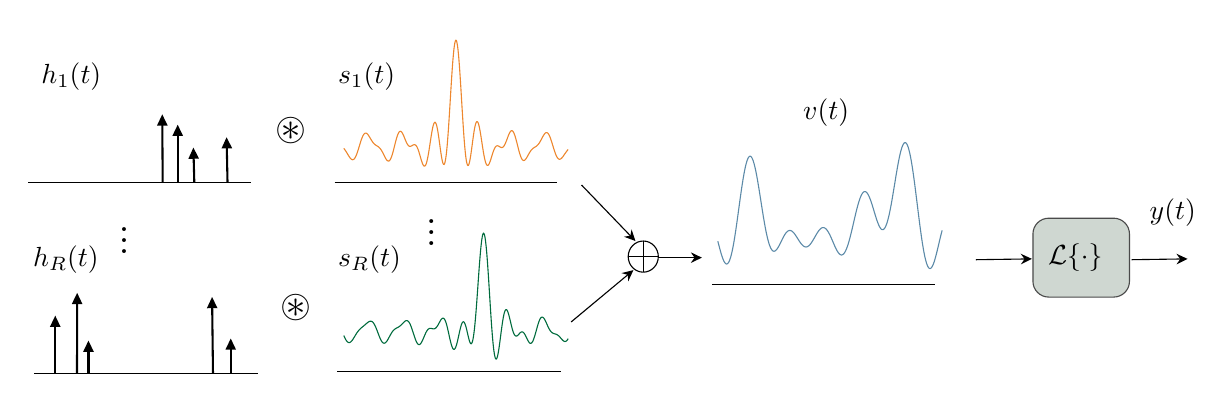
\begin{tikzpicture}[x=0.75pt,y=0.75pt,yscale=-1,xscale=1]
%uncomment if require: \path (0,172); %set diagram left start at 0, and has height of 172

%Straight Lines [id:da42079222359818846] 
\draw    (57.93,71) -- (165.5,71) ;
%Shape: Boxed Line [id:dp9855841335838222] 
\draw [line width=0.75]    (129.95,70.98) -- (129.95,45.98) ;
\draw [shift={(129.95,42.98)}, rotate = 90] [fill={rgb, 255:red, 0; green, 0; blue, 0 }  ][line width=0.08]  [draw opacity=0] (5.36,-2.57) -- (0,0) -- (5.36,2.57) -- cycle    ;
%Straight Lines [id:da9053021816658018] 
\draw [line width=0.75]    (122.71,71) -- (122.52,41) ;
\draw [shift={(122.5,38)}, rotate = 89.63] [fill={rgb, 255:red, 0; green, 0; blue, 0 }  ][line width=0.08]  [draw opacity=0] (5.36,-2.57) -- (0,0) -- (5.36,2.57) -- cycle    ;
%Straight Lines [id:da6648976924921457] 
\draw [line width=0.75]    (137.95,70.98) -- (137.58,57) ;
\draw [shift={(137.5,54)}, rotate = 88.49] [fill={rgb, 255:red, 0; green, 0; blue, 0 }  ][line width=0.08]  [draw opacity=0] (5.36,-2.57) -- (0,0) -- (5.36,2.57) -- cycle    ;
%Straight Lines [id:da5266947861725098] 
\draw [line width=0.75]    (153.95,70.98) -- (153.56,52) ;
\draw [shift={(153.5,49)}, rotate = 88.83] [fill={rgb, 255:red, 0; green, 0; blue, 0 }  ][line width=0.08]  [draw opacity=0] (5.36,-2.57) -- (0,0) -- (5.36,2.57) -- cycle    ;
%Straight Lines [id:da9439510016771822] 
\draw    (60.93,163) -- (168.5,163) ;
%Shape: Boxed Line [id:dp6681929173819516] 
\draw [line width=0.75]    (86.95,162.98) -- (86.95,150) ;
\draw [shift={(86.95,147)}, rotate = 90] [fill={rgb, 255:red, 0; green, 0; blue, 0 }  ][line width=0.08]  [draw opacity=0] (5.36,-2.57) -- (0,0) -- (5.36,2.57) -- cycle    ;
%Straight Lines [id:da6516144259229273] 
\draw [line width=0.75]    (70.95,162.98) -- (70.95,137.98) ;
\draw [shift={(70.95,134.98)}, rotate = 90] [fill={rgb, 255:red, 0; green, 0; blue, 0 }  ][line width=0.08]  [draw opacity=0] (5.36,-2.57) -- (0,0) -- (5.36,2.57) -- cycle    ;
%Straight Lines [id:da7298105615379362] 
\draw [line width=0.75]    (81.43,163) -- (81.49,127) ;
\draw [shift={(81.5,124)}, rotate = 90.11] [fill={rgb, 255:red, 0; green, 0; blue, 0 }  ][line width=0.08]  [draw opacity=0] (5.36,-2.57) -- (0,0) -- (5.36,2.57) -- cycle    ;
%Straight Lines [id:da32933274297788384] 
\draw [line width=0.75]    (146.95,162.98) -- (146.54,129) ;
\draw [shift={(146.5,126)}, rotate = 89.31] [fill={rgb, 255:red, 0; green, 0; blue, 0 }  ][line width=0.08]  [draw opacity=0] (5.36,-2.57) -- (0,0) -- (5.36,2.57) -- cycle    ;
%Straight Lines [id:da3162669830150253] 
\draw [line width=0.75]    (155.5,163) -- (155.5,149) ;
\draw [shift={(155.5,146)}, rotate = 90] [fill={rgb, 255:red, 0; green, 0; blue, 0 }  ][line width=0.08]  [draw opacity=0] (5.36,-2.57) -- (0,0) -- (5.36,2.57) -- cycle    ;
%Straight Lines [id:da6544073952598419] 
\draw [color={rgb, 255:red, 0; green, 0; blue, 0 }  ,draw opacity=1 ]   (205.5,71) -- (312.5,71) ;
%Straight Lines [id:da8775446294620928] 
\draw [color={rgb, 255:red, 0; green, 0; blue, 0 }  ,draw opacity=1 ]   (206.93,162) -- (314.5,162) ;
%Straight Lines [id:da8658741007955231] 
\draw    (324.5,72) -- (348.42,96.84) ;
\draw [shift={(350.5,99)}, rotate = 226.08] [fill={rgb, 255:red, 0; green, 0; blue, 0 }  ][line width=0.08]  [draw opacity=0] (5.36,-2.57) -- (0,0) -- (5.36,2.57) -- (3.56,0) -- cycle    ;
%Straight Lines [id:da927735437828485] 
\draw    (319.5,138) -- (347.2,114.92) ;
\draw [shift={(349.5,113)}, rotate = 140.19] [fill={rgb, 255:red, 0; green, 0; blue, 0 }  ][line width=0.08]  [draw opacity=0] (5.36,-2.57) -- (0,0) -- (5.36,2.57) -- (3.56,0) -- cycle    ;
\draw   (347,106.5) .. controls (347,102.36) and (350.25,99) .. (354.25,99) .. controls (358.25,99) and (361.5,102.36) .. (361.5,106.5) .. controls (361.5,110.64) and (358.25,114) .. (354.25,114) .. controls (350.25,114) and (347,110.64) .. (347,106.5) -- cycle ; \draw   (347,106.5) -- (361.5,106.5) ; \draw   (354.25,99) -- (354.25,114) ;
%Straight Lines [id:da27108196110843386] 
\draw    (361.5,107) -- (379.5,107) ;
\draw [shift={(382.5,107)}, rotate = 180] [fill={rgb, 255:red, 0; green, 0; blue, 0 }  ][line width=0.08]  [draw opacity=0] (5.36,-2.57) -- (0,0) -- (5.36,2.57) -- (3.56,0) -- cycle    ;
%Rounded Rect [id:dp17940737225962167] 0.7, 0.75, 0.71
\draw  [color={rgb, 255:red, 74; green, 74; blue, 74 }  ,draw opacity=1 ][fill={rgb, 1:red, 0.7; green, 0.75; blue, 0.71 }  ,fill opacity=0.62 ] (542,95.6) .. controls (542,91.4) and (545.4,88) .. (549.6,88) -- (580.9,88) .. controls (585.1,88) and (588.5,91.4) .. (588.5,95.6) -- (588.5,118.4) .. controls (588.5,122.6) and (585.1,126) .. (580.9,126) -- (549.6,126) .. controls (545.4,126) and (542,122.6) .. (542,118.4) -- cycle ;
%Straight Lines [id:da09645578299438706] 
\draw    (589.5,108) -- (613.5,107.65) ;
\draw [shift={(616.5,107.61)}, rotate = 179.17] [fill={rgb, 255:red, 0; green, 0; blue, 0 }  ][line width=0.08]  [draw opacity=0] (5.36,-2.57) -- (0,0) -- (5.36,2.57) -- (3.56,0) -- cycle    ;
% Plotting does not support converting to Tikz
% Plotting does not support converting to Tikz
%Straight Lines [id:da797089328299941] 
\draw [color={rgb, 255:red, 0; green, 0; blue, 0 }  ,draw opacity=1 ]   (387.43,119.85) -- (495,119.85) ;
% Plotting does not support converting to Tikz
%Straight Lines [id:da9570209190184586] 
\draw    (514.5,108) -- (538.5,107.65) ;
\draw [shift={(541.5,107.61)}, rotate = 179.17] [fill={rgb, 255:red, 0; green, 0; blue, 0 }  ][line width=0.08]  [draw opacity=0] (5.36,-2.57) -- (0,0) -- (5.36,2.57) -- (3.56,0) -- cycle    ;

% Text Node
\draw (63,12) node [anchor=north west][inner sep=0.75pt]  [font=\normalsize]  {$h_{1}( t)$};
% Text Node
\draw (59,100) node [anchor=north west][inner sep=0.75pt]  [font=\normalsize]  {$h_{R}( t)$};
% Text Node
\draw (176,38.34) node [anchor=north west][inner sep=0.75pt]  [font=\Large]  {$\circledast$};
% Text Node
\draw (178,123.46) node [anchor=north west][inner sep=0.75pt]  [font=\Large]  {$\circledast$};
% Text Node
\draw (100,83.4) node [anchor=north west][inner sep=0.75pt]  [font=\LARGE]  {$\vdots $};
% Text Node
\draw (430,29.4) node [anchor=north west][inner sep=0.75pt]  [font=\normalsize]  {$v( t)$};
% Text Node
\draw (248,79.4) node [anchor=north west][inner sep=0.75pt]  [font=\LARGE]  {$\vdots $};
% Text Node
\draw (206,12) node [anchor=north west][inner sep=0.75pt]  [font=\normalsize]  {$s_{1}( t)$};
% Text Node
\draw (206,100) node [anchor=north west][inner sep=0.75pt]  [font=\normalsize]  {$s_{R}( t)$};
% Text Node
\draw (548,99) node [anchor=north west][inner sep=0.75pt]  [font=\normalsize]  {$\mathcal{L}\{\cdot\}$};
% Text Node
\draw (597,77.4) node [anchor=north west][inner sep=0.75pt]  [font=\normalsize]  {$y(t)$};



% = ===== Curve ===== g1(t) 

\begin{axis}[
width=5cm,
height=3.5cm,
xticklabels=none,
 yticklabels=none,
 xtick=\empty,
 ytick=\empty,
 axis line style={draw=none},
 xshift=5.25cm,yshift=-0.1cm,
 ]
\addplot[
    domain=-20:20,
    samples=500, 
    color=cadmiumorange,
]{0.1*(-5*sin(2*deg(x))/x+cos(deg(x)-3))};
\end{axis}

% = ===== Curve ===== gr(t)
\begin{axis}[
width=5cm,
height=3.5cm,
xticklabels=none,
 yticklabels=none,
 xtick=\empty,
 ytick=\empty,
 axis line style={draw=none},
 xshift=5.25cm,yshift=2.35cm,
 ]
\addplot[
    domain=-20:20,
    samples=500, 
    color=cadmiumgreen,
]{0.1*(-5*sin(2*deg(x-5))/(x-5)+cos(deg(x)-1))};
\end{axis}
% = ===== Curve ===== y(t)
\begin{axis}[
width=5cm,
height=3.5cm,
xticklabels=none,
 yticklabels=none,
 xtick=\empty,
 ytick=\empty,
 axis line style={draw=none},
 xshift=10cm,yshift=1.2cm,
 ]
\addplot[
    domain=-20:20,
    samples=500, 
    color=airforceblue,
]{-15*sin(deg(x+14))/(x+14)+cos(deg(x)-1)-10*sin(deg(x-7))/(x-7)+cos(deg(x)-1) -20*sin(deg(x-13))/(x-13) };
\end{axis}



\end{tikzpicture}
}
    
    \caption{An illustration of the mathematical model of \ac{GB2D} problem. Every user transmits waveform $s_r(t)$ over channel $h_r(t)$ involves $s_r$ multi-path. Afterward, the sum of all these convolved signals is received by $v(t)$.   }
    \label{fig:system}
\end{figure*}


% || ==================== ||
  The linear observation of the mixture model in~\eqref{eq:measure} appears in a variety of applications, including asynchronous over-the-air computation~\cite{SaeedBlind2022}, super-resolution single-molecule imaging~\cite{three-dimensionalsuper,SaeedBinary2020},  multi-user multipath channel estimation~\cite{jung2017blind,daei2023blind}, blind calibration in multi-channel sampling systems~\cite{vetterli2010multichannel,SayyariBlind2021} and integrated (radar) sensing and communications (ISAC)~\cite{liu2020joint}. 
  
For instance, in ISAC applications, radar or communication users or even ISAC transmitters transmit signals in the same time-frequency resource towards a common ISAC receiver, and the task of the common ISAC receiver is not only to estimate the parameters of the radar targets but also to estimate the data of communications users. Specifically,
$s_r(t), r\in [R]$ in the model \eqref{eq:mymodel} can be some radar transmitters, and it can be represented by the data of some communications users in the uplink. Similarly, $h_r(t)$ can be the communications channels or the sensing channels ($r\in[R]]$), which can also have some correlations with each other \cite{liu2020joint}. The task of the dual-functional common ISAC receiver is to estimate the continuous radar parameters (such as delays, velocity, angle of arrival, etc.) encoded in $h_r(t), r\in [R]$  and subsequently to separate the radar and communications signals and channels occupying the same time-bandwidth resources.

  In the past few years, notable progress has been made in addressing blind deconvolution problems, with a particular emphasis on sparse signals composed of a single tone, i.e., $R=1$  \cite{jain2017non,ahmed2013blind,ling2015self,candes2013phaselift}. The common approach considers the continuous channel parameters (delays in \eqref{eq:mymodel}) to lie on predefined domains of grids which can then be estimated using the well-established methods of compressed sensing such as $\ell_1$ minimization. However, the predefined grids might not match the true continuous-index values of parameters which leads to basis mismatch issues that can degrade the performance of blind deconvolution.   
 Motivated by recent advances in continuous parameter estimation \cite{candes2014towards}, a blind deconvolution method is developed in \cite{chi2016guaranteed} to recover a continuous parameter in case of $R=1$. In this paper, we deal with a general and more challenging model that is a mixture of blind deconvolution problems, and the transmitted signals $s_r(t)$'s are totally different from each other and do not follow a particular channel model. Moreover, for the sake of generality and practicality, we also consider the availability of having a compressed linear combination of the data samples instead of observing the whole samples as in~\cite{Jacome2020DualBlind}. 
 
Specifically,  GB2D exploits a lifting technique to convert the demixing of nonlinear problems into the demixing of high-dimensional matrices that contain continuous parameters. Then, we propose a tractable convex optimization problem that considers the features of these matrices to recover the channel parameters, i.e., $\overline{\tau}_r^R, r=1,\ldots, P_R$'s. A least square problem is then developed to estimate the transmitted waveforms, i.e., $s_r(t)$'s.  Our method is built upon the assumption that the transmitted signals by different users lie in known low-dimensional subspaces.   In addition to the aforementioned contributions, we provide the conditions under which the solution to GB2D becomes unique and optimal. Finally, we verify the effectiveness of GB2D through simulation results, demonstrating that GB2D succeeds in recovering the continuous parameters as well as the transmitted messages with a sufficient number of samples.

% it can recover all sparse spike signals and accurately estimate the transmitted waveforms.


The rest of the paper is organized as follows.  In Section~\ref{sec.model}, the problem formulation is formalized. In Section~\ref{sec.proposed}, we provide the GB2D method, which includes the convex optimization and dual problem to localize the spikes. Section~\ref{sec.simulations} verifies the performance of GB2D through simulations. Lastly, the paper is concluded in Section~\ref{sec.conclusion}.


The paper shows vectors and matrices in boldface lower-and upper-case letters, respectively.  For vector $\bm{x}\in\mathbb{C}^N$ and matrix $\bm{X}\in\mathbb{C}^{N_1\times N_2}$, the norms $\ell_2$ is defined as $\|\bm{x}\|_2:= \sqrt{\sum_{i=1}^n|x(i)|^2}$. 
We further use $\odot$ to show Hadamard products (element-wise products). $\mathscr{T} : \mathbb{C}^N \to \mathbb{C}^{N\times N}$ is the Toeplitz lifting operator that maps the input vector $\bm{x}$  into  a Toeplitz matrix $\bm{M}=\mathscr{T}(\bm{x})$, such that $\bm{M}_{(i,j)} = \bm{x}_{|i+j-1|}$. Also, $\mathscr{T}^{\dagger}$ is the inverse Toeplitz operator. We use $\langle \cdot, \cdot \rangle$ to show the inner product operator where  
for two arbitrary matrices $\bm{A}, \bm{B}$, i.e., $\langle \bm{A}, \bm{B}\rangle$ represents ${\rm Tr} (\bm{B}^{\mathsf  H}\bm{A})$ and for two continuous functions $f(t)$ and $g(t)$ it means $\int_{-\infty}^{\infty}f(t)g(t)dt$ by $\langle f(t), g(t) \rangle$. The notation $\bm{A}\succeq \bm{0}$ means $\bm{A}$ is a positive semidefinite matrix.

 


 % ## =========================== ##
 \section{Problem Formulation}\label{sec.model}
 % ## =========================== ##

Assuming the measured signal $y(t)$ is square-integrable in Lebesgue’s sense, we can expand it as $y(t):=  \sum_{m=1}^M y_m \varphi_m(t)$  where  $\varphi_n$s  are compact support basis functions for $t\in [0, T]$ that are orthonormal, i.e., 
 %--------------
 \begin{align}
    \langle\varphi_i(t), \varphi_j(t) \rangle :=  \int_{-\infty}^{\infty}\varphi_i(t)\varphi_j(t) dt  = \delta_{i-j},     
 \end{align}
%--------------
 where $\delta_{i-j}$ is the discrete delta Dirac function. Then, $m$-th sample of the signal in~\eqref{eq:measure}, can be written as 
 %--------------
 \begin{align}
    \label{eq:innerVL}
     \nonumber y_m &= \langle \mathcal{L}\{v(t)\}, \varphi_m \rangle = \langle v(t), \underbrace{\mathcal{L}^*\{\varphi_m \}}_{\ell_{m}(t)}\rangle \\ 
     \nonumber & = \langle \mathscr{F}^*\mathscr{F}\{v(t)\}, \ell_{m}(t)\rangle = \langle \mathscr{F}\{v(t)\}, \mathscr{F}\{\ell_{m}(t)\}\rangle \\
     & = \langle V(f), L_m(f)\rangle,
 \end{align}
 %--------------
where $\mathscr{F}(\cdot)$ denotes linear Fourier operator, and $V(f)$ and $L_m(f)$ are the Fourier transform of $v(t)$ and $\ell_m(t)$, respectively. Let $\{s_r(t)\}_{r=1}^R$ be the transmitted waveforms whose spectrum lie in the interval $[-B,B]$. Taking the Fourier transform of~\eqref{eq:mymodel}, we have the following.
%--------------
 \begin{align} \label{eq.Yf}
V(f)=\sum_{r=1}^{R}H_r(f)S_r(f), ~\forall f\in [-B,B],
 \end{align}   
%--------------
 where $V(f)$, $H_r(f)$, and $S_r(f)$ are the Fourier transform of $v(t)$, $h_r(t)$, and $s_r(t)$, respectively. Substituting \eqref{eq.Yf} into \eqref{eq:innerVL}, we obtain
 %--------------
  \begin{align}
     \nonumber y_m = \sum_{r=1}^{R} \langle H_r(f)S_r(f), L_m(f)\rangle  ,
 \end{align}
 %--------------
 By uniformly sampling \eqref{eq.Yf} at $N$ points $f_n=Bn/\lfloor (N-1)/2\rfloor,~n= -\lceil (N-1)/2\rceil, \ldots, \lfloor (N-1)/2\rfloor$ or $n=0,\ldots, N-1$ provided that $BT\le \lfloor (N-1)/2\rfloor$, we reach
  %--------------
 \begin{align}\label{eq.sampledmodel1}
  y_m =  \langle \bm{\ell}_m, \sum_{r=1}^R \bm{h}_r\odot \bm{s}_r \rangle = \langle \bm{\ell}_m, \bm{v} \rangle,
  % v_n=\sum_{r=1}^Rx_n^rg_n^r=\sum_{r=1}^{R}\sum_{k=1}^{S_r}g_k^r{\rm e}^{-j2\pi n \tau_k^r \frac{BT}{M} }g_n^r,
 \end{align}
  %--------------
where 
 %--------------
\begin{align}
    \bm{h}_r & = [H(f_1),\ldots,H(f_N)]^{\mathsf{T}}, \\
     \bm{s}_r & = [S(f_1),\ldots,S(f_N)]^{\mathsf{T}}, \\ 
     \bm{\ell}_m & = [L_m(f_1),\ldots,L_m(f_N)]^{\mathsf{T}}, \\
     \bm{v} & =  [V(f_1),\ldots,V(f_N)]^{\mathsf{T}}.
\end{align}
%--------------
Note that to set $N$ as small as possible without loss of generality, we choose $N= 2BT + 1$.
The relation in \eqref{eq.sampledmodel1} can be represented in a matrix form as
  %--------------
 \begin{align}
 \bm{y}=\bm{L}\sum_{r=1}^R \bm{h}_r\odot \bm{s}_r,
 \end{align}
  %--------------
 where $\bm{y}=[y_{1},...,y_{M}]^{\mathsf{T}}$ and $\bm{L} = [\bm{\ell}_1,\ldots, \bm{\ell}_M]^{\mathsf{T}} \in \mathbb{C}^{M\times N}$. Recall that $h_r(t) = \sum_{k=1}^{P_r}g_k^r\delta(t-\tau_k^r)$, then 
\begin{align}
    \label{eq.sampledmodel2}
   \bm{y} = \bm{L}\sum_{r=1}^R \sum_{k=1}^{P_r}g_k^r \bm{a}(\tau_k^r)\odot \bm{s}_r,
\end{align}
 where $\bm{a}(\tau):=[1,{\rm e}^{-j2\pi\tau}, \ldots ,{\rm e}^{-j2\pi(N-1)\tau}]^{\mathsf{T}}.$

 
 
 Our goal is to recover $\tau_k^r$s, $g_k^r$s, and $\bm{s}_r$s from the observation vector $\bm{y}\in\mathbb{C}^{M}$. It is unavoidable to have scaling ambiguities for recovering $\bm{s}_r$'s and $\bm{h}_r$'s because of any $\alpha_r\in\mathbb{C}\setminus\{0\}$, we have
  %--------------
 \begin{align}
 \bm{y}= \bm{L}\sum_{r=1}^R\alpha_r\bm{h}_r\odot \frac{\bm{s}_r}{\alpha_r}.
 \end{align}
  %--------------
 Without further constraints, the problem \eqref{eq.sampledmodel1} is highly ill-posed because the number of samples $M$ is much smaller than the  number of unknowns $\mathcal{O}(N\sum_{r=1}^R P_r)$. To alleviate this challenge, we make the assumption that each $\bm{s}_r$ lies in a low-dimensional subspace, i.e.,
  %--------------
 \begin{align}\label{eq.subspace_assumption}
 \bm{s}_r=\bm{C}_r\bm{x}_r,
 \end{align} 
  %--------------
 where $\bm{C}_r:=[\bm{c}_{1}^r, \ldots, \bm{c}_{N}^r]^{\mathsf{T}}\in\mathbb{C}^{N\times K_r}$,
  is a known basis of the subspace with $N\gg K_r$ and $\bm{x}_r\in\mathbb{C}^{K_r}$ is unknown for BS. For example, in wireless communications, $\bm{x}_r$  and $\bm{C}_r$ are the message vector of the $r$-th user and its corresponding codebook matrix, respectively.  Without loss of generality, we assume that the messages are $\ell_2$ normalized, i.e., $\|\bm{x}_r\|_2=1$. In the next section, we present the GB2D method for demixing the measured signals by putting some subspace constraints on the transmitted vectors as in \eqref{eq.subspace_assumption}. 
  We also define the separation between the delays of $r$-th channel as
\begin{align}
\Delta_r:=\min_{k\neq q}|\tau^r_k-\tau^r_q|,
\end{align} 
and the minimum separation between all users by $\Delta:=\min_{i} \Delta_r$. The absolute value in the latter definition is evaluated as wrap-around distance on the unit circle.

% || ==================== ||
 \begin{figure}[!t]
\centering
 \begin{tikzpicture} 

 \begin{scope}[spy using outlines={rectangle, magnification=5,
   width=1.6cm,height=1.6cm,connect spies}]
    \begin{axis}[
        width=0.5\textwidth,
        height=6cm,
        xmin=0, xmax=1,
        ymin=1e-3, ymax=1,
        legend style={nodes={scale=0.55, transform shape}, at={(0.3,0.95)}}, 
        ticklabel style = {font=\footnotesize},
        %legend pos=west,
        ymajorgrids=true,
        xmajorgrids=true,
        grid style=dashed,
        grid=both,
        grid style={line width=.1pt, draw=gray!10},
        major grid style={line width=.2pt,draw=gray!30},
    ]
    \addplot[ smooth,
             thin,
        color=chestnut,
        %mark=star,
        %mark options = {rotate = 180},
        line width=0.9pt,
        %mark size=3pt,
        ]
    table[x=t,y=D1]
    {Data/PolyDual3.dat};
\addplot[ smooth,
             thin,
        color=airforceblue,
        %mark=star,
        %mark options = {rotate = 180},
        line width=0.9pt,
        %mark size=3pt,
        ]
    table[x=t,y=D2]
    {Data/PolyDual3.dat};
    \addplot[ 
        color=cadmiumorange,
        mark=star,
        dashed,
        %mark options = {rotate = 180},
        line width=1pt,
        mark size=1pt,
        ]
    table[x=t,y=X1]
    {Data/PolyDual3.dat};
    \addplot[ 
        color=azure,
        mark=star,
        dashed,
        %mark options = {rotate = 180},
        line width=0.5pt,
        mark size=0.5pt,
        ]
    table[x=t,y=X2]
    {Data/PolyDual3.dat};
    \legend{$(\mathcal{B}^*\bm{\lambda})_1$, $(\mathcal{B}^*\bm{\lambda})_2$,$\tau_1$,$\tau_2$};
     \path (0.639, 0.99) coordinate (X);
    \end{axis}
    \spy [black] on (X) in node (zoom) [left] at ([xshift=2.5cm,yshift=-0.5cm]X);
    \end{scope}
\end{tikzpicture}

  \caption{Delay estimation via dual polynomials with order  $N=64$ for $K=2$ and $P_1=2,P_2=1$ with $M_1=M_2 =5$.  }
   \label{fig:Daul}
\end{figure}

% || ==================== ||

% ## =========================== ##
\section{Proposed Method}\label{sec.proposed}
% ## =========================== ##
 In this section, we introduce the main idea GB2D method and propose a convex optimization to recover all the channel parameters $\overline{\tau}_r^R, r=1, \ldots, P_r$s and transmitted waveforms $s_r(t)$s with general known codebook matrices $\bm{C}_r$s.  Invoking the subspace assumption \eqref{eq.subspace_assumption},  $n$-th Fourier samples of signal $v(t)$ can be written as 
 %--------------
 \begin{align}\label{eq.sampledmodel3}
 V(f_n)&= \sum_{r=1}^R\sum_{k=1}^{P_r}g_k^r\bm{e}_n^{\mathsf{T}}\bm{a}(\tau_k^r)\bm{x}_r^{\mathsf{T}}\bm{c}^r_n,
 \end{align}
 %--------------
 where $\bm{e}_n$ stands for the $n$-th column of $\bm{I}_{N}$. Let $\bm{X}_r=\sum_{k=1}^{P_r} g_k^r\bm{x}_r\bm{a}(\tau_k^r)^{\mathsf{T}}\in\mathbb{C}^{K_r\times N}$. Using the lifting trick \cite{ling2015self}, the measurements $V(f_n), n\in [N]$ in \eqref{eq.sampledmodel3} can be written as
 %--------------
 \begin{align}\label{eq:SamplesInner}
 &V(f_n)=\sum_{r=1}^R\sum_{k=1}^{P_r}g_k^r {\rm Tr}\Big(\bm{c}^r_n\bm{e}_n^{\mathsf{T}}\bm{a}(\tau_k^r)\bm{x}_r^{\mathsf{T}}\Big)=\sum_{r=1}^R\big\langle \bm{X}_r, \bm{c}^r_n\bm{e}_n^{\mathsf{T}}\big\rangle.
 \end{align} 
 %--------------
 Writing in matrix form, we have $\bm{v}=\mathcal{C}(\bm{\mathcal{X}}),$ where $\bm{\mathcal{X}}:=(\bm{X}_r)_{r=1}^R\in \bigoplus_{r=1}^r\mathbb{C}^{K_r\times N}$ is the matrix tuple of interest and $\mathcal{C}$ is the linear measurement mapping defined as
 %--------------
 \begin{align*}
 \bigoplus_{r=1}^R\mathbb{C}^{K_r\times N}\rightarrow \mathbb{C}^N,~~ \bm{\mathcal{Z}}\rightarrow \Bigg(\sum_{r=1}^R\big\langle \bm{Z}_r, \bm{c}^r_n\bm{e}_n^{\mathsf{T}}\big\rangle\Bigg)_{n=1}^{N}.	
 \end{align*}
 %--------------
Then, by defining $ \mathcal{B} := \bm{L}\mathcal{C}$, the measurements $\bm{y}$ reads to
 %--------------
\begin{align}\label{eq:measure_model1}
    \bm{y}  =  \mathcal{B}(\mathcal{X}). 
\end{align} 
%--------------
 
 In model~\eqref{eq.sampledmodel3}, the number of delays $\{P_r\}_{r=1}^R$ (e.g., in a multipath channel in multi-user wireless systems) is small. 
 Thus, we define the atomic norm~\cite{chandrasekaran2012convex}
 %--------------
 \begin{align}\label{eq.atomic_def}
 &\|\bm{Z}\|_{\mathcal{A}_r}:=\inf\{t>0: \bm{Z}\in t{\rm conv}(\mathcal{A}_r)\}\nonumber\\
 &=\inf_{\substack{c_k, \tau_k\\\|{\bm{x}_k}\|_2=1}}\Big\{\sum_{k}|c_k|:~\bm{Z}=\sum_{k}c_k \bm{x}_r\bm{a}(\tau_k)^{\mathsf{T}}  \in\mathbb{C}^{K_r\times N} \Big\}
 \end{align}
 %--------------
 associated with the atoms
 %--------------
 \begin{align}
 &\mathcal{A}_r=\big\{\bm{x}\bm{a}(\tau)^{\mathsf{T}}: \tau\in[0,1), \|\bm{x}\|_2=1, \bm{x}\in\mathbb{C}^{K_r} \big\}, r\in [R].
 \end{align}
 %--------------
  The atomic norm $\|\bm{X}_r\|_{\mathcal{A}_r}$ can be regarded as the best convex alternative for the smallest number of atoms $\mathcal{A}_r$ needed to represent a signal $\bm{X}_r$. Hence, we are interested in recovering the matrix tuple $\bm{\mathcal{X}}:=(\bm{X}_r)_{r=1}^R$ by motivating its atomic sparsity by solving the following optimization problem. 
 %--------------
 \begin{align}\label{eq.primalprob}
 \min_{\bm{\mathcal{Z}}=(\bm{Z}_r)_{r=1}^R} ~\sum_{r=1}^{R}\|\bm{Z}_r\|_{\mathcal{A}_r}\quad 
 \bm{y}_{M\times 1}=\mathcal{B}(\bm{\mathcal{Z}}).	
 \end{align} 
 %--------------
Finding the optimal parameters in \eqref{eq.primalprob} is not an easy task because it involves an infinite-dimensional variable optimization due to the continuity of the set. Alternatively, we can solve the dual problem explained in the next section.   

% || ==================== ||
\begin{figure*}[!t]
\centering
\subfigure[]{\label{Fig(a):Circ}
 \begin{tikzpicture} 
 \begin{scope}[spy using outlines={rectangle, magnification=4,
   width=1.6cm,height=1.6cm,connect spies}]
    \begin{axis}[
        width=6cm,
        height=6cm,
        xmin=-1, xmax=1,
        ymin=-1, ymax=1,
        legend style={nodes={scale=0.65, transform shape}, at={(0.7,0.92)}}, 
        ticklabel style = {font=\footnotesize},
        %legend pos=west,
        ymajorgrids=true,
        xmajorgrids=true,
        grid style=dashed,
        grid=both,
        grid style={line width=.1pt, draw=gray!10},
        major grid style={line width=.2pt,draw=gray!30},
    ]
    \addplot[only marks,
        color=chestnut,
        mark=star,
        %mark options = {rotate = 180},
        line width=0.75pt,
        mark size=2pt,
        ]
    table[x=X1,y=Y1]
    {Data/Sim1.dat};
   \addplot[only marks,
        color=chestnut,
        mark=o,
        %mark options = {rotate = 180},
        line width=0.75pt,
        mark size=2pt,
        ]
    table[x=TX1,y=TY1]
    {Data/Sim2.dat};

    \draw[azure,thick,dashed] (axis cs:0,0) circle [radius=1];
    
    % =============
    \addplot[only marks,
        color=airforceblue,
        mark=star,
        mark options = {rotate = 180},
        line width=0.75pt,
        mark size=2pt,
        ]
    table[x=X2,y=Y2]
    {Data/Sim1.dat};
    \addplot[only marks,
        color=airforceblue,
        mark=o,
        %mark options = {rotate = 180},
        line width=0.75pt,
        mark size=2pt,
        ]
    table[x=TX2,y=TY2]
    {Data/Sim2.dat};
    % =============
    \addplot[only marks,
        color=black,
        mark=star,
        line width=0.75pt,
        mark size=2pt,
        ]
    table[x=X3,y=Y3]
    {Data/Sim1.dat};
    \addplot[only marks,
        color=black,
        mark=o,
        %mark options = {rotate = 180},
        line width=0.75pt,
        mark size=2pt,
        ]
    table[x=TX3,y=TY3]
    {Data/Sim2.dat};
    % =============
    \addplot[only marks,
        color=cadmiumorange,
        mark=star,
        line width=0.75pt,
        mark size=2pt,
        ]
    ttable[x=X4,y=Y4]
    {Data/Sim1.dat};
    \addplot[only marks,
        color=cadmiumorange,
        mark=o,
        %mark options = {rotate = 180},
        line width=0.75pt,
        mark size=2pt,
        ]
    table[x=TX4,y=TY4]
    {Data/Sim2.dat};
    \legend{Estimated channel, True delays};
     \path (0.75, -0.62) coordinate (X);
    \end{axis}
    \spy [black] on (X) in node (zoom) [left] at ([xshift=-0.5cm,yshift=1cm]X);
    \end{scope}
\end{tikzpicture}
}
% =====================
\subfigure[]{\label{Fig(b):Circ}
\begin{tikzpicture} 
    \begin{axis}[
       % xlabel={$\cos(t)$},
        %ylabel={$\sin(t)$},
        %label style={font=\tiny},
        %title = {\small $f(\bm{x}) = \prod_{k=1}^Kx_k$},
        % legend cell align={left},
        width=6cm,
        height=6cm,
        xmin=-1, xmax=1,
        ymin=-1, ymax=1,
        %xtick={-1, -0.5, 0, 0.5, 1},
        %ytick={0, 20, 40, 60, 80, 100},
        legend style={nodes={scale=0.65, transform shape}, at={(0.7,0.9)}}, 
        ticklabel style = {font=\footnotesize},
        %legend pos=west,
        ymajorgrids=true,
        xmajorgrids=true,
        grid style=dashed,
        grid=both,
        grid style={line width=.1pt, draw=gray!10},
        major grid style={line width=.2pt,draw=gray!30},
    ]
    \addplot[only marks,
        color=chestnut,
        mark=star,
        %mark options = {rotate = 180},
        line width=1pt,
        mark size=3pt,
        ]
    table[x=TEX1,y=TEY1]
    {Data/resultR3L5N128NEW.dat};
   \addplot[only marks,
        color=chestnut,
        mark=o,
        %mark options = {rotate = 180},
        line width=1pt,
        mark size=3pt,
        ]
    table[x=TX1,y=TY1]
    {Data/resultR3L5N128NEW.dat};

    \draw[azure,thick,dashed] (axis cs:0,0) circle [radius=1];
    
    % =============
    \addplot[only marks,
        color=airforceblue,
        mark=star,
        mark options = {rotate = 180},
        line width=1pt,
        mark size=3pt,
        ]
    table[x=TEX2,y=TEY2]
    {Data/resultR3L5N128NEW.dat};
    \addplot[only marks,
        color=airforceblue,
        mark=o,
        %mark options = {rotate = 180},
        line width=1pt,
        mark size=3pt,
        ]
    table[x=TX2,y=TY2]
    {Data/resultR3L5N128NEW.dat};
    % =============
    \addplot[only marks,
        color=black,
        mark=star,
        line width=1pt,
        mark size=3pt,
        ]
    table[x=TEX3,y=TEY3]
    {Data/resultR3L5N128NEW.dat};
    \addplot[only marks,
        color=black,
        mark=o,
        %mark options = {rotate = 180},
        line width=1pt,
        mark size=3pt,
        ]
    table[x=TX3,y=TY3]
    {Data/resultR3L5N128NEW.dat};
    \legend{Estimated channel, True delays};
    \end{axis}
\end{tikzpicture}
}
% =====================
\subfigure[]{\label{Fig(c):Circ}
\begin{tikzpicture} 
    \begin{axis}[
       % xlabel={$\cos(t)$},
        %ylabel={$\sin(t)$},
        %label style={font=\tiny},
        %title = {\small $f(\bm{x}) = \prod_{k=1}^Kx_k$},
        % legend cell align={left},
        width=6cm,
        height=6cm,
        xmin=-1, xmax=1,
        ymin=-1, ymax=1,
        %xtick={-1, -0.5, 0, 0.5, 1},
        %ytick={0, 20, 40, 60, 80, 100},
        legend style={nodes={scale=0.65, transform shape}, at={(0.7,0.95)}}, 
        ticklabel style = {font=\footnotesize},
        %legend pos=west,
        ymajorgrids=true,
        xmajorgrids=true,
        grid style=dashed,
        grid=both,
        grid style={line width=.1pt, draw=gray!10},
        major grid style={line width=.2pt,draw=gray!30},
    ]
    \addplot[only marks,
        color=chestnut,
        mark=star,
        %mark options = {rotate = 180},
        line width=1pt,
        mark size=3pt,
        ]
    table[x=X1,y=Y1]
    {Data/resultR2L16N64NEW.dat};
   \addplot[only marks,
        color=chestnut,
        mark=o,
        %mark options = {rotate = 180},
        line width=1pt,
        mark size=3pt,
        ]
    table[x=TX1,y=TY1]
    {Data/resultR2L16N64NEW.dat};

    \draw[azure,thick,dashed] (axis cs:0,0) circle [radius=1];
    
    % =============
    \addplot[only marks,
        color=airforceblue,
        mark=star,
        mark options = {rotate = 180},
        line width=1pt,
        mark size=3pt,
        ]
    table[x=X2,y=Y2]
    {Data/resultR2L16N64NEW.dat};
    \addplot[only marks,
        color=airforceblue,
        mark=o,
        %mark options = {rotate = 180},
        line width=1pt,
        mark size=3pt,
        ]
    table[x=TX2,y=TY2]
    {Data/resultR2L16N64NEW.dat};
    % =============
    \legend{Estimated channel, True delays};
    \end{axis}
\end{tikzpicture}
}
  \caption{Performance of \ac{GB2D}. Fig~\ref{Fig(a):Circ} shows the channel estimation for the case where for $K=4$ users and $P_1=\cdots=P_4=3$, form $N=200$ samples and the message size $M_k=5$ for $k\in [4]$. Fig~\ref{Fig(b):Circ} depict the performance of \ac{GB2D} for $K=3$ with $P_1=3,P_2=2,P_3 = 1$ from $N=128$ samples. Fig~\ref{Fig(c):Circ} shows  the output of \ac{GB2D} for the case $M_k=16$ and $M=64$. Each signal is shown with a different color code. 
  }
   \label{fig:Plor}
\end{figure*}

% || ==================== |

%=================
\begin{prop}\label{prop.optimality}
Denote the set of multipath's delays of $h_r(t)$ as $\mathcal{P}_r:=\{\tau_k^r\}_{k=1}^{P_r}$. The solution $\widehat{\bm{\mathcal{X}}}=(\widehat{\bm{X}}_r)_{r=1}^R$ of \eqref{eq.primalprob} is unique if there exists a vector $\bm{\lambda}=[\lambda_{1}, \ldots, \lambda_{N}]^{\mathsf{T}}\in\mathbb{C}^N$ such that the vector-valued dual polynomials 
%--------------
\begin{align}\label{eq.Qi}
\bm{q}_r(\tau)=(\mathcal{B}^*\bm{\lambda})_r\bm{a}^*(\tau)= \sum_{n=1}^{N}\lambda_n {\rm e}^{j2\pi n \tau} \bm{c}_n^r\in\mathbb{C}^{k_r}, 
\end{align}
%--------------
for $r \in [R]$, satisfy the conditions
%--------------
\begin{align}
&\bm{q}_r(\tau_k)={\rm sgn}({c_k^{i}})\bm{x}_r~\forall \tau_k\in \mathcal{P}_r,~ r\in [R]\label{eq.supp_cond}\\
&\|\bm{q}_r(\tau)\|_2<1~~\forall \tau \in [0,1)\setminus \mathcal{P}_r,~ r\in [R]\label{eq.offsupp_cond}
\end{align}
%--------------
 \end{prop}
%=================
\begin{proof}
See Appendix \ref{proof.optimality}.
\end{proof}




\begin{corl}
The dual polynomial $\bm{q}_r(\tau)$ only depends on its corresponding codebook, i.e.,   $\bm{C}_r$. Therefore, in the case where all users employ the same codebook matrix, all users have a common subspace, i.e., $\bm{C}_r = \bm{C} \in \mathbb{C}^{N\times K}$,  all the atomic norms in \eqref{eq.primalprob} can be replaced with only one atom and its dual polynomial. 
\end{corl}            


% ## =========================== ##
 \subsection{Channel estimation via Dual Problem}
% ## =========================== ##
Before proceeding with the dual problem, let us define the dual polynomial of the atomic norm in the sequel.  In particular, the dual atomic norm $\|\cdot\|_{\mathcal{A}_r}^{\mathsf{d}}$ at an arbitrary point $\bm{Z}\in \mathbb{C}^{k_r\times N}$ is defined as
%--------------
\begin{align}\label{eq.dualnorm1}
&\|\bm{Z}\|_{\mathcal{A}_r}^{\mathsf{d}}:=\sup_{\|\bm{X}\|_{\mathcal{A}_r}\le 1}{\rm Re}\big\{\langle \bm{Z}, \bm{X} \rangle\big\}=\sup_{\substack{\tau\in [0,1)\\\|\bm{x}\|_2=1}}{\rm Re}\big\{\langle \bm{Z}, \bm{x}\bm{a}(\tau)^{\mathsf{T}} \rangle\big\} \nonumber\\
&=\sup_{\substack{\tau\in [0,1)\\\|\bm{x}\|_2=1}}{\rm Re}\big\{\langle \bm{x}, \bm{Z}\bm{a}^*(\tau) \rangle\big\}=\sup_{\tau\in [0,1)}\|\bm{Z}\bm{a}^*(\tau)\|_2.
\end{align}
%--------------
Then, by assigning the Lagrangian vector $\bm{\lambda}\in\mathbb{C}^N$ to the equality constraint of \eqref{eq.primalprob}, we have
%--------------
\begin{align}\label{eq.lagran1}
&L(\bm{\mathcal{Z}},\bm{\lambda})=\inf _{\bm{\mathcal{Z}}\in\bigoplus_{r=1}^R\mathbb{C}^{K_r\times N}}\Big[\sum_{r=1}^R\|\bm{Z}_r\|_{\mathcal{A}_r}+\langle \bm{\lambda},\bm{y}-\mathcal{B}(\bm{\mathcal{Z}}) \rangle\Big]\nonumber\\
&\langle \bm{\lambda},\bm{y}\rangle+\sum_{r=1}^R\inf_{\bm{Z}_r\in\mathbb{C}^{K_r\times N}}\Big[\|\bm{Z}_r\|_{\mathcal{A}_r}-\langle (\mathcal{B}^*\bm{\lambda})_r, \bm{Z}_r \rangle\Big],
\end{align}
%--------------
where we used that $\langle \mathcal{B}^*\bm{\lambda}, \bm{\mathcal{Z}}\rangle=\sum_{r=1}^R\langle (\mathcal{B}^*\bm{\lambda})_r, \bm{Z}_r\rangle.$
By using H\"{o}lder's inequality, \eqref{eq.lagran1} becomes equivalent to
%--------------
\begin{align}
\nonumber L(\bm{\mathcal{Z}},\bm{\lambda})&=\langle  \bm{\lambda},\bm{y}\rangle
\\
& +\sum_{r=1}^R\inf_{\bm{Z}_r\in\mathbb{C}^{K_r\times N}}\Big[\|\bm{Z}_r\|_{\mathcal{A}_r}(1-\|(\mathcal{B}^*\bm{\lambda})_r\|_{\mathcal{A}_r}^{\mathsf{d}})\Big].
\end{align}
%--------------
Solving the latter optimization problem, we obtain 
%--------------
\begin{align}
&L(\bm{\mathcal{Z}},\bm{\lambda})= \begin{cases}
\langle \bm{\lambda},\bm{y}\rangle,&~~ \|(\mathcal{B}^*\bm{\lambda})_r\|_{\mathcal{A}_r}^{\mathsf{d}}\le 1,~ r \in [R] \\
-\infty, &{\rm otherwise.}
\end{cases}	
\end{align}
%--------------
By transforming implicit constraints into explicit ones, the dual problem becomes
%--------------
\begin{align}\label{eq.lagran2}
\max_{\bm{\lambda}\in\mathbb{C}^{N}}~\langle \bm{\lambda},\bm{y}\rangle \quad {\rm s.t.}\quad 
\|(\mathcal{B}^*\bm{\lambda})_r\|_{\mathcal{A}_r}^{\mathsf{d}}\le 1,\quad 
r \in [R],
\end{align}
%--------------
 where $\mathcal{B}^*:\mathbb{C}^{M}\rightarrow \bigoplus_{r=1}^R\mathbb{C}^{K_r\times N}$ denotes the adjoint operator of $\mathcal{B}$ and $\mathcal{B}^*\bm{\lambda}:=((\mathcal{B}^*\bm{\lambda})_r)_{r=1}^R$ is a matrix tuple where the $r$-th matrix is given by $(\mathcal{B}^*\bm{\lambda})_r=\sum_{n=1}^{N}\lambda_n\bm{c}^r_n\bm{e}_n^{\mathsf{T}}.$
 %--------------
Maximization in \eqref{eq.lagran2} can also be presented in SDP format as 
 %--------------
\begin{equation}\label{prob.sdp}
    \begin{aligned}
    &\bm{\lambda}^* = \underset{\substack{\bm{\lambda}\in\mathbb{C}^{N}\\ \bm{Q}\in \mathbb{C}^{N\times N}}}{\rm argmax}~~{\rm Re}\big\{\langle \bm{\lambda}, \bm{y}\rangle\big\}\\
    &~~~~{\rm s.t.}~~
    \begin{bmatrix}
        \bm{Q}&(\mathcal{B}^{*}(\bm{\lambda}))_r\\
        (\mathcal{B}^{*}(\bm{\lambda}))_r^{\mathsf{H}}&\bm{I}_T
    \end{bmatrix}\succeq \bm{0}, \quad r \in [R],\\
    & ~~~~~~\langle \mathscr{T}({\bm{e}_q}), \bm{Q}  \rangle=1_{q=0}, \quad q=-N+1,..., N-1,
    \end{aligned}
\end{equation}	
 %--------------
 where $\mathscr{T}$ shows the Toeplitz structure. 
Maximization in \eqref{prob.sdp} is a convex problem; therefore,  it can be efficiently solved using the CVX toolbox \cite{grant2014cvx}.  Let $\hat{\bm{\lambda}}$ be the solution to the dual problem in~\eqref{eq.lagran2},
then the spikes can be localized by the peaks of the following term $ \hat{\mathcal{T}}_r = \Big\{\tau \in [0,1) | \big\|  (\mathcal{B}^* \hat{\bm{\lambda}})_r \bm{a}(\tau) \big\|_2=1 \Big\}.$

% To obtain the messages of users, we replace the estimated delays into\eqref{eq:measure_model1} which to the following overdetermined linear system of equations. 
 For instance, an example of this channel estimation is depicted in Fig~\ref{fig:Daul} for a case with $R=2$. 
 
 To recover the message vector and the channel amplitudes corresponding to the $r$-th user, we form  $\widehat{\bm{Z}}_r=\sum_{k}\widehat{g}_k^r \widehat{\bm{x}}_r\bm{a}(\widehat{\tau}_k^r)^{\mathsf{T}}$. Let $\widehat{\bm{g}}^r:=[\widehat{g}_1^r, \ldots,\widehat{g}_{P_r}^r]^{\mathsf{T}}$. Then, the rank one matrix $\widehat{\bm{x}}_r$ can be estimated as $\widehat{\bm{x}}_r\widehat{\bm{g}}^{r\mathsf{T}}=\widehat{\bm{Z}}_r\bm{A}^{(r)\dagger}$ where $\bm{A}^{(r)}:=[\bm{a}(\widehat{\tau}_1^r), \ldots,\bm{a}(\widehat{\tau}_1^{P_r})]^\mathsf{T}$. By using the assumption $\|\widehat{\bm{x}}_r\|_2=1$ and taking singular value decomposition, we can find $|\widehat{\bm{x}}_r|$ and $|\widehat{\bm{g}}^r|$ for $r=1, \ldots, R$.
 
 % and multiplying the left-hand side of the latter equation by $\widehat{\bm{x}}_r^T$, we can estimate $\widehat{\bm{c}}^r=\bm{A}^{{(r)\dagger}^T}\widehat{\bm{Z}}_r\widehat{\bm{x}}_r, r=1,..., S_R$. Then, by knowing $|\widehat{c}_i^{r}|$, we can estimate the absolute value of each element of the channel corresponding to the $r$-th user, i.e., $|\widehat{\bm{x}}_r|$.
 % rank one matrix $\hat{\bm{Z}}_r = \bm{u}_rS_r\bm{v}^{\mathsf{H}}$  and set $\hat{\bm{x}}_r =  \sqrt{S_r}\bm{u}_r$ and $\bm{d}_k: = \sum_{k}c_k^{r}\bm{a}(\tau_k^{r}) =  \sqrt{S_r}\bm{u}_r$. Finally, the amplitudes of $x_r(t)$ is obtained by least square solution i.e. $\bm{c}^{r} = \bm{A}^{(r)\dagger} \bm{d}_k$ where  $\bm{A} \in \mathbb{C}$ is complex matrix whose $k$-th column is $\bm{a}(\tau_k^{r})$.
 
% {\scriptsize{
%      \begin{align}
%          \begin{bmatrix}
%               \bm{e}_{-2M}^T
%               \bm{a}(\hat{\tau}_1^1)
%               {\bm{b}_{-2M}^1}^T
%               &\hdots&\bm{e}_{-2M}^T\bm{a}(\widehat{\tau}_{s_r}^r){\bm{b}_{-2M}^r}^T\\
%               \vdots&\ddots&\vdots\\
%            \bm{e}_{2M}^T
%               \bm{a}(\hat{\tau}_1^1)
%               {\bm{b}_{2M}^1}^T
%              &\hdots&\bm{e}_{2M}^T\bm{a}(\widehat{\tau}_{s_r}^r){\bm{b}_{2M}^r}^T\\
%          \end{bmatrix} \begin{bmatrix}
%              c_1^1 \bm{x}_1\\
%              \vdots\\
%              c_{s_1}^1 \bm{x}_1\\
%              \vdots\\
%              c_1^r \bm{x}_r\\
%              \vdots\\
%              c_{s_r}^r \bm{x}_r\\
%          \end{bmatrix}=\begin{bmatrix}
%              y(-2M)\\
%              \vdots\\
%              y(2M)
%          \end{bmatrix}
%      \end{align}}
% }

% || ==================== ||
\input{Figures/Fig_Massage}
% || ==================== |



% ## =========================== ##
\section{Simulation Results}\label{sec.simulations}
% ## =========================== ##



This section evaluates the optimization performance in \eqref{eq.lagran2} for different channel delays and message lengths. Then numerical experiments are implemented using MATLAB CVX Toolbox \cite{grant2014cvx}.  The delays' locations are generated uniformly at random with the minimum separation $\Delta\geq \frac{1}{N}$ to be smaller than what we theoretically expected.  The basis of low  
dimensional tall matrix $\bm{C}_r\in \mathbb{C}^{ N \times K_r}$ is generated uniformly at random for $r\in [R]$ from normal distribution $\mathcal{N}(0,1)$. The messages $\bm{x}_r, r=1, \ldots, R$ are generated \textit{i.i.d} and uniformly at random  from the unit sphere. It is worth mentioning that if there is some sort of coordination on the values of transmitted messages (e.g., positiveness) between users and BS, then the transmitted messages can be uniquely and unambiguously estimated by the proposed method.   



For the first case,  we set $R=4$ with $P_1=\cdots=P_4=3$ from $N=200$ samples, and the filter size $K_r=5$ for $r\in [4]$. Also, the sensing matrix $\bm{L}$ is set to be identity, i.e., $\bm{L}=\bm{I}_N$. Then, the results are depicted in Fig~\ref{Fig(a):Circ}. Fig~\ref{Fig(a):Circ} shows that it can recognize two almost co-located sources. In Fig~\ref{Fig(b):Circ}, we repeat this experiment for $R=3$ with $K_1=3,K_2=2,K_3=1$ from $N=128$ samples.  


For the last case, we check the stability of the algorithm regarding a larger filter size $K_r=16$ with $N=128$ samples and the effect of the sensing matrix with $M=64$. Indeed, the sensing matrix does the sub-sampling uniform by selecting half of the samples  in Fig~\ref{Fig(c):Circ}.

We observe that all the cases are successfully recovered by GB2D for a sufficient number of samples $N$. 

Finally, we evaluate the performance of the GB2D method for massage recovery in Fig~\ref{fig:Mas}.  Fig~\ref{fig:Mas} depicts the means square error (MSE) of recovered massages  by the GB2D for the number of samples $N$. We set both transmitted signals to have a massage of size $16$, i.e.,  $K_1 = K_2= 16$ and, also, the number of multipath is set to $P_1 = 2$ and $P_2 = 3$ for massage $\bm{x}_1$ and $\bm{x}_2$, respectively. Note that increasing the number of samples at BS leads to lower massage recovery MSE errors.  


The results of this section show that for different numbers of multipath and various sizes of massages, GB2D  can simultaneously recover massages and estimate multipath channels with a sufficient number of samples.  


% ## =========================== ##
\section{Conclusion}\label{sec.conclusion}
% ## =========================== ##

The focus of our paper was to explore the possibility of simultaneous blind deconvolution and demixing when multiple users send their messages through multiple channels and a BS receives a linear combination of multiple convolved channels that are made up of a few scaled and delayed continuous Dirac spikes. Specifically, the measurements we worked with were a compressed version of the collective sum of these convolved signals with unknown amplitudes.
The main goal was to find these unknown channel delay parameters from only one vector of observations. Since this problem is inherently highly challenging to solve, we overcome this issue by restricting the domain of the transmitted signals to some known low-dimensional subspaces while we have a separation condition on the Dirac spikes. Afterward, we proposed a semidefinite programming optimization to recover the channel delays and the messages of different users simultaneously from one observed vector.
For future works, we will provide the performance guarantee of the proposed method by obtaining the required sample complexity that one needs for perfect recovery of the continuous parameters and the transmitted waveforms.
 



\appendix

\section{Proof of Proposition \ref{prop.optimality}}\label{proof.optimality}

Any $\bm{\lambda}\in\mathbb{C}^N$ satisfying \eqref{eq.supp_cond} and \eqref{eq.offsupp_cond} is a feasible point in the dual problem \eqref{eq.lagran2}. Recall that $\bm{\mathcal{X}}=(\bm{X}_r)_{r=1}^R$ is the matrix tuple of interests where $\bm{X}_r=\sum_{k=1}^{P_r}g_k^r\bm{x}_r\bm{a}(\tau_k^r)^{\mathsf{T}}$. It holds that
%--------------
\begin{align}\label{eq.rel1}
&\sum_{r=1}^R\|\bm{X}_r\|_{\mathcal{A}_r}\ge \sum_{r=1}^R\|\bm{X}_r\|_{\mathcal{A}_r}\|(\mathcal{B}^*\bm{\lambda})_r\|_{\mathcal{A}_r}^{\mathsf{d}}\ge\nonumber\\
&\sum_{r=1}^R\langle (\mathcal{B}^*\bm{\lambda})_r, \bm{X}_r \rangle=\sum_{r=1}^R\langle (\mathcal{B}^*\bm{\lambda})_r, \sum_{k=1}^{P_r}g_k^r\bm{x}_r\bm{a}(\tau_k^r)^{\mathsf{T}} \rangle=\nonumber\\
&\sum_{r=1}^R\sum_{k=1}^{P_r}{\rm Re}\Big\{{g_k^r}^*\langle (\mathcal{B}^{\ast}\bm{\lambda})_r, \bm{x}_r\bm{a}(\tau_k^r)^{\mathsf{T}} \rangle \Big\} \nonumber\\
&=\sum_{r=1}^R\sum_{k=1}^{P_r}{\rm Re}\Big\{{g_k^r}^*\langle \bm{Q}_r(\tau_k^r), \bm{x}_r \rangle\Big\},
\end{align}
%--------------
where the second inequality is due to H\"{o}lder's inequality, and the last equalities are due to the definition of $\bm{Q}_r(\tau_k^r)$ in \eqref{eq.Qi}. We proceed \eqref{eq.rel1} by using conditions \eqref{eq.supp_cond} and \eqref{eq.offsupp_cond}:
%--------------
\begin{align}\label{eq.rel2}
&\sum_{r=1}^R\|\bm{X}_r\|_{\mathcal{A}_r}\ge \sum_{r=1}^R\sum_{k=1}^{P_r}{\rm Re}\Big\{{g_k^r}^*\langle \frac{1}{\|\bm{x}_r\|_2^2}{\rm sgn}(g_k^r)\bm{x}_r, \bm{x}_r \rangle\Big\}  \nonumber\\
&\sum_{r=1}^R\sum_{k=1}^{P_r}|g_k^r|\ge\sum_{r=1}^R\|\bm{X}_r\|_{\mathcal{A}_r},
\end{align}
%--------------
where we used the definition of atomic norm \eqref{eq.atomic_def} in the last step. From \eqref{eq.rel1} and \eqref{eq.rel2}, we find that 
$\langle \bm{\lambda}, \mathcal{B}\bm{\mathcal{X}}\rangle=\sum_{r=1}^R\|\bm{X}_r\|_{\mathcal{A}_r}$. Since the pair $(\bm{\mathcal{X}}, \bm{\lambda})$ is primal-dual feasible, we reach the conclusion that $\bm{\mathcal{X}}$ is an optimal solution of \eqref{eq.primalprob} and $\bm{\lambda}$ is an optimal solution of \eqref{eq.lagran2} by strong duality. For proving uniqueness, suppose $\widehat{\bm{\mathcal{X}}}:=(\widehat{\bm{X}}_r)_{r=1}^R$ is another optimal solution of \eqref{eq.primalprob} where $\widehat{\bm{X}}_r=\sum_{\widehat{\tau}_k^r\in \widehat{\mathcal{P}}_r}\widehat{g}_k^r\widehat{\bm{x}}_r\bm{a}(\widehat{\tau}_k^r)^{\mathsf{T}}$. If $\widehat{\bm{\mathcal{X}}}$ and $\bm{\mathcal{X}}$ have the same set of delays, i.e., $\widehat{\mathcal{P}}_r=\mathcal{P}_r,~\forall~r \in [R]$, we then have $\widehat{\bm{\mathcal{X}}}=\bm{\mathcal{X}}$ since the set of atoms building $\bm{\mathcal{X}}$ are linearly independent. If there exists some $\widehat{\tau}_k^r\notin \mathcal{P}_r$, then we can expand term $\langle \bm{\lambda}, \mathcal{B}\widehat{\bm{\mathcal{X}}}\rangle$ as follows 
%--------------
\begin{align}\label{eq.rel3}
&\sum_{r=1}^R\langle (\mathcal{B}^*\bm{\lambda})_r, \widehat{\bm{X}}_r\rangle=
\sum_{r=1}^R \sum_{k}{\rm Re}\Big\{{\overset{*}{\widehat{g}_k^r}}\langle (\mathcal{B}^*\bm{\lambda})_r, \widehat{\bm{x}}_r\bm{a}(\widehat{\tau}_k^r)^{\mathsf{T}} \rangle\Big\}=\nonumber\\
&	\sum_{r=1}^R\Big[\sum_{\widehat{\tau}_k^r\in \mathcal{P}_r}{\rm Re}\Big\{{\overset{*}{\widehat{g}_k^r}}
\langle\bm{Q}_r(\widehat{\tau}_k^r),\widehat{\bm{x}}_r \rangle\Big\}+\hspace{-8pt}\sum_{\widehat{\tau}_k^r\notin \mathcal{P}_r}{\rm Re}\Big\{{\overset{*}{\widehat{g}_k^r}}
\langle\bm{Q}_r(\widehat{\tau}_k^r),\widehat{\bm{x}}_r \rangle\Big\}\Big]\le\nonumber\\
&\sum_{r=1}^R\Big[\sum_{\widehat{\tau}_k^r\in \mathcal{P}_r}|\widehat{g}_k^r|
\|\bm{Q}_r(\widehat{\tau}_k^r)\|_2\|\widehat{\bm{x}}_r\|_2 +\sum_{\widehat{\tau}_k^r\notin \mathcal{P}_r}|\widehat{g}_k^r|
\|\bm{Q}_r(\widehat{\tau}_k^r)\|_2\|\widehat{\bm{x}}_r\|_2\Big]\nonumber\\
&<\sum_{r=1}^R\Big[\sum_{\widehat{\tau}_k^r\in \mathcal{P}_r}|\widehat{g}_k^r|
 +\sum_{\widehat{\tau}_k^r\notin \mathcal{P}_r}|\widehat{g}_k^r|\Big]=\sum_{r=1}^R|\widehat{g}_k^r|=\sum_{r=1}^R\|\widehat{\bm{X}}_r\|_{\mathcal{A}_r},
\end{align}
%--------------
where we used the conditions \eqref{eq.supp_cond} and \eqref{eq.offsupp_cond}. The relation \eqref{eq.rel3} contradicts strong duality; hence $\bm{\mathcal{X}}$ is the unique optimal solution of \eqref{eq.primalprob}.


\bibliographystyle{IEEEtran}
\bibliography{Ref}

% \bibliographystyle{ieeetr}



\end{document}
